\chapter{M\'odulo de Citas (Agenda)}

\section{Descripci\'on General}

El m\'odulo de citas proporciona una agenda diaria con gesti\'on completa
de citas veterinarias. Incluye un flujo de estados que modela el ciclo de
vida real de una consulta: desde la programaci\'on hasta el check-out.

\section{M\'aquina de Estados}

Las citas siguen una m\'aquina de estados con 7 estados:

\begin{verbatim}
scheduled --> confirmed --> checked_in --> in_exam --> checked_out
    |             |
    +--> cancelled+--> cancelled
                      no_show
\end{verbatim}

\begin{itemize}[leftmargin=*]
    \item \textbf{scheduled:} Cita programada inicialmente.
    \item \textbf{confirmed:} Confirmada por el cliente.
    \item \textbf{checked\_in:} Cliente lleg\'o a la cl\'{\i}nica.
    \item \textbf{in\_exam:} Mascota en consulta.
    \item \textbf{checked\_out:} Consulta finalizada.
    \item \textbf{cancelled:} Cancelada (desde scheduled o confirmed).
    \item \textbf{no\_show:} Cliente no se present\'o.
\end{itemize}

Cada transici\'on es unidireccional hacia adelante. Los estados
\texttt{cancelled}, \texttt{checked\_out} y \texttt{no\_show} son
terminales.

\section{Server Actions}

\subsection{getAppointments --- Consulta con M\'ultiples Joins}

\begin{lstlisting}[style=typescript, caption={getAppointments - Joins con pacientes, clientes y usuarios}]
export async function getAppointments(date?: string) {
  const clinicId = await getCurrentClinicId();
  const conditions = [eq(schema.appointments.clinicId, clinicId)];
  if (date) {
    conditions.push(eq(schema.appointments.date, date));
  }

  const rows = await db
    .select({
      id: schema.appointments.id,
      date: schema.appointments.date,
      startTime: schema.appointments.startTime,
      endTime: schema.appointments.endTime,
      type: schema.appointments.type,
      status: schema.appointments.status,
      notes: schema.appointments.notes,
      room: schema.appointments.room,
      patientId: schema.appointments.patientId,
      patientName: schema.patients.name,
      patientSpecies: schema.patients.species,
      clientId: schema.appointments.clientId,
      clientName: schema.clients.name,
      vetId: schema.appointments.vetId,
      vetName: schema.users.firstName,
      vetLastName: schema.users.lastName,
    })
    .from(schema.appointments)
    .innerJoin(schema.patients,
      eq(schema.appointments.patientId, schema.patients.id))
    .innerJoin(schema.clients,
      eq(schema.appointments.clientId, schema.clients.id))
    .leftJoin(schema.users,
      eq(schema.appointments.vetId, schema.users.id))
    .where(conditions.length > 0 ? and(...conditions) : undefined)
    .orderBy(schema.appointments.date, schema.appointments.startTime);

  return rows;
}
\end{lstlisting}

\subsection{createAppointment --- Notificaci\'on Autom\'atica}

\begin{lstlisting}[style=typescript, caption=createAppointment con notificacion]
export async function createAppointment(data: AppointmentInput) {
  const clinicId = await getCurrentClinicId();
  await db.insert(schema.appointments).values({
    clinicId,
    patientId: data.patientId,
    clientId: data.clientId,
    vetId: data.vetId,
    date: data.date,
    startTime: data.startTime,
    endTime: data.endTime,
    type: data.type as any,
    status: 'scheduled',
    notes: data.notes || null,
    room: data.room || null,
  });

  // Obtener nombres para la notificacion
  const [patient, client] = await Promise.all([
    db.select({ name: schema.patients.name })
      .from(schema.patients)
      .where(eq(schema.patients.id, data.patientId))
      .then(r => r[0]),
    db.select({ name: schema.clients.name })
      .from(schema.clients)
      .where(eq(schema.clients.id, data.clientId))
      .then(r => r[0]),
  ]);

  const vetIds = data.vetId ? [data.vetId] : [];
  await notifyNewAppointment({
    clientName: client?.name ?? 'Cliente',
    patientName: patient?.name ?? 'Mascota',
    date: data.date,
    time: data.startTime.slice(0, 5),
    vetIds,
  });

  revalidatePath('/appointments');
}
\end{lstlisting}

\subsection{updateAppointmentStatus --- Transiciones R\'apidas}

\begin{lstlisting}[style=typescript, caption=updateAppointmentStatus]
export async function updateAppointmentStatus(
  id: number, status: string
) {
  await db
    .update(schema.appointments)
    .set({ status: status as any })
    .where(eq(schema.appointments.id, id));

  revalidatePath('/appointments');
  revalidatePath(`/appointments/${id}`);
}
\end{lstlisting}

\section{P\'aginas}

\subsection{Agenda Diaria (/appointments)}

\begin{itemize}[leftmargin=*]
    \item Vista diaria con fecha seleccionable via \texttt{?date=YYYY-MM-DD}.
    \item Navegaci\'on entre fechas con botones ``$<$'', ``Hoy'', ``$>$''.
    \item Cada cita muestra: hora, paciente, due\~no, tipo, sala y veterinario.
    \item Acciones r\'apidas de cambio de estado (2 acciones por cita).
    \item Colores sem\'anticos seg\'un el estado.
\end{itemize}

\subsection{Creaci\'on (/appointments/new)}

\begin{itemize}[leftmargin=*]
    \item Formulario con selectores dependientes:
    \item Al elegir un due\~no, se cargan sus mascotas via
          \texttt{GET /api/patients/by-client/[id]}.
    \item Al elegir una mascota, se autocompleta el due\~no.
    \item Selector de veterinarios desde \texttt{GET /api/users/vets}.
    \item Campos: fecha, hora inicio, hora fin, tipo, sala, notas.
\end{itemize}

\subsection{Detalle (/appointments/[id])}

\begin{itemize}[leftmargin=*]
    \item Informaci\'on completa: fecha, hora, tipo, estado, sala.
    \item Datos del paciente y due\~no.
    \item Veterinario asignado.
    \item Panel de transici\'on de estado seg\'un flujo permitido.
\end{itemize}

\section{API Routes}

\begin{lstlisting}[style=typescript, caption=APIs para selectores dependientes]
// GET /api/patients/by-client/[id]
// GET /api/users/vets
\end{lstlisting}

Estas APIs permiten la carga din\'amica de selectores en los formularios
del lado del cliente, optimizando la experiencia de usuario.

\begin{figure}[H]
    \centering
    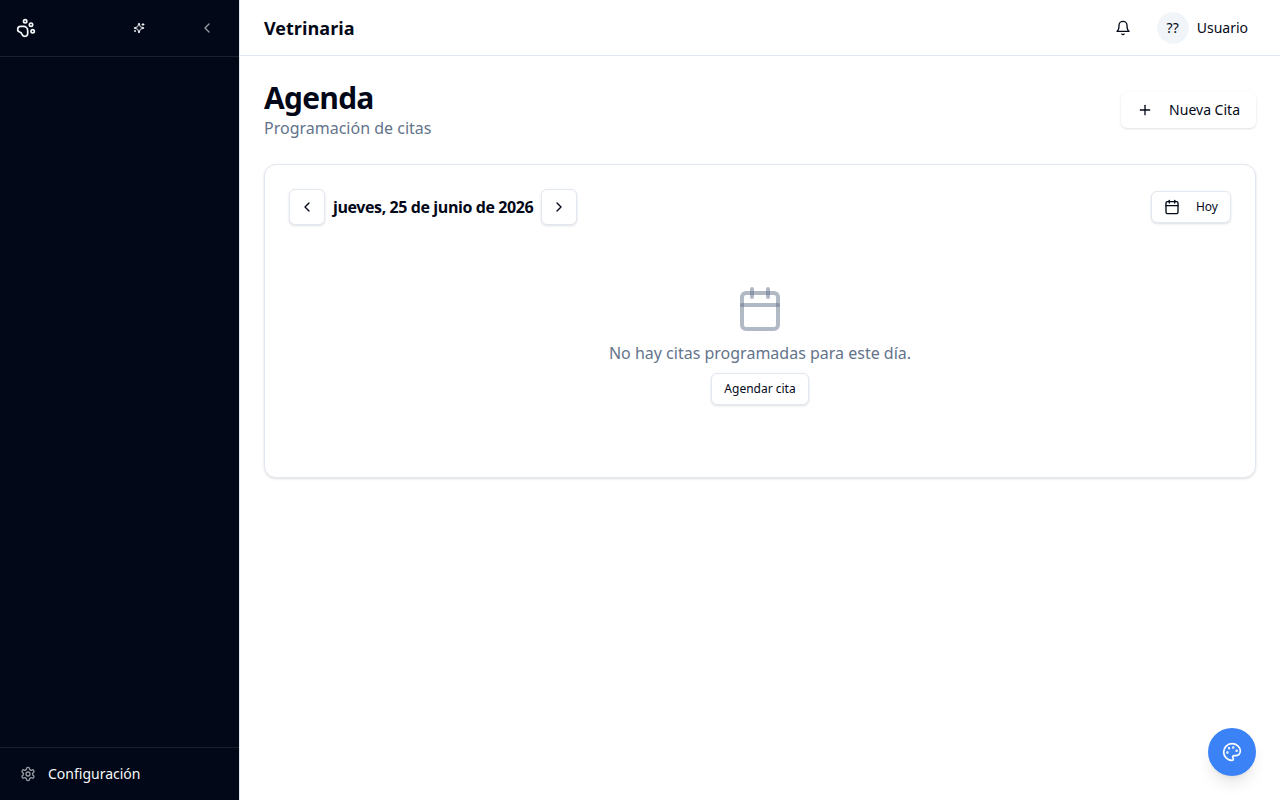
\includegraphics[width=\textwidth]{img/vet-appointments.png}
    \caption{Agenda diaria con citas, estados y acciones rapidas}
    \label{fig:citas}
\end{figure}
